% Transplant-ready introduction and motivation snippet for the main paper.
% This is a fragment, not a full LaTeX document.

\section{Introduction}

Why do some workers become entrepreneurs only when paid employment is
unavailable, and what does that imply for policy? This question lies at the
center of debates over labor markets, small business, and social insurance, yet
necessity entrepreneurship is difficult to identify in observed data. The
object of interest is inherently counterfactual. A worker is a necessity
entrepreneur if they enter business ownership when a viable employment
relationship is unavailable, but would prefer wage work if such a relationship
were available. Standard startup data do not reveal that counterfactual. The
same observed entry may reflect entrepreneurial comparative advantage,
temporary self-employment during job search, insurance against labor-market
risk, or a response to job loss. These cases are unlikely to have the same
implications for firm scale, growth potential, or welfare.

Empirical work has approached this identification problem in two main ways. One
uses stated motives. The Global Entrepreneurship Monitor (GEM) provides
nationally representative survey evidence on why individuals start businesses
and shows that necessity-type motives are quantitatively important even in the
United States. In weighted U.S. APS microdata for 2019--2021, the share of
early-stage entrepreneurs endorsing the motive "to earn a living because jobs
are scarce" is 40.9 percent in 2019, 49.6 percent in 2020, and 45.7 percent in
2021. At the same time, 68.3 percent, 64.7 percent, and 73.4 percent,
respectively, endorse the motive of building great wealth or very high income.
The coexistence of these responses is informative rather than contradictory: it
shows that necessity-type considerations are common, but also that necessity
and opportunity signals need not be mutually exclusive within the same
entrepreneurial spell. The most recent U.S. GEM report points in the same
direction, documenting a sharp rise in job-scarcity motives between 2021 and
2023 \citep{gem_us_report_2024}. Cross-country evidence is equally suggestive.
The GEM 2015/16 global report shows that 78 percent of entrepreneurs in
innovation-driven economies are opportunity-motivated, and that the ratio of
improvement-driven opportunity to necessity entrepreneurship is much higher in
richer economies than in factor-driven ones
\citep{kelley_singer_herrington_2016}. Related evidence on entrepreneurial
aspirations likewise suggests that the motives behind entry vary systematically
with development \citep{chivers_2017}.

A second empirical strategy classifies entrepreneurs by observed labor-market
status. \citet{fairlie_fossen_2019} define opportunity entrepreneurship as
entry from employment and necessity entrepreneurship as entry from
non-employment, and show that the two components have different cyclical
properties and different growth orientation. \citet{fairlie_2013} and
\citet{fossen_2021} similarly find that business creation is more
countercyclical on margins associated with unemployment-driven and
unincorporated entry. These classifications are tractable and informative, but
they are not equivalent to the counterfactual object of interest. A worker who
expects separation may start a business while still employed and appear
opportunity-driven in the data, while a non-employed worker may enter
temporarily while continuing to search and appear necessity-driven even when
their long-run entrepreneurial comparative advantage is high.

This paper takes survey-based and status-based classifications seriously, but
treats them as proxies rather than definitions. We instead adopt a structural,
state-contingent definition. An opportunity entrepreneur is an agent who
chooses business ownership whether they enter the period employed or
non-employed. A necessity entrepreneur is an agent who chooses business
ownership only when they lack an employment relationship. The distinction maps
directly into occupational choice, does not require taking survey answers
literally, and does not equate necessity mechanically with entry from
non-employment. We embed that distinction in a quantitative occupational-choice
framework with entrepreneurial ability, human capital, search frictions, and
unemployment insurance so that the model speaks jointly to entry, entrant type,
and firm scale.

Business-cycle evidence is useful in this setting because downturns compress
outside options, but recession patterns are best viewed as motivation rather
than definition. Our empirical side evidence is consistent with that view. In
U.S. business counts by employment size, the Great Recession is associated with
relative resilience at the zero-employee margin and contraction across employer
establishments. Between 2007 and 2010, zero-employee establishments rise by
about 1.9 percent, while establishments with 1--4 employees fall by 3.6
percent, establishments with 5--19 employees fall by 2.6 percent, and
establishments with 20 or more employees fall by 5.8 percent. Aggregate counts
move little because growth at the zero-employee margin offsets declines among
employer establishments. The natural interpretation is not that recessions
simply create more firms, but that weaker outside options shift activity toward
low-scale business ownership. Figure~\ref{fig:us_business_counts_by_size}
illustrates this compositional pattern directly.

\begin{figure}[t]
\centering
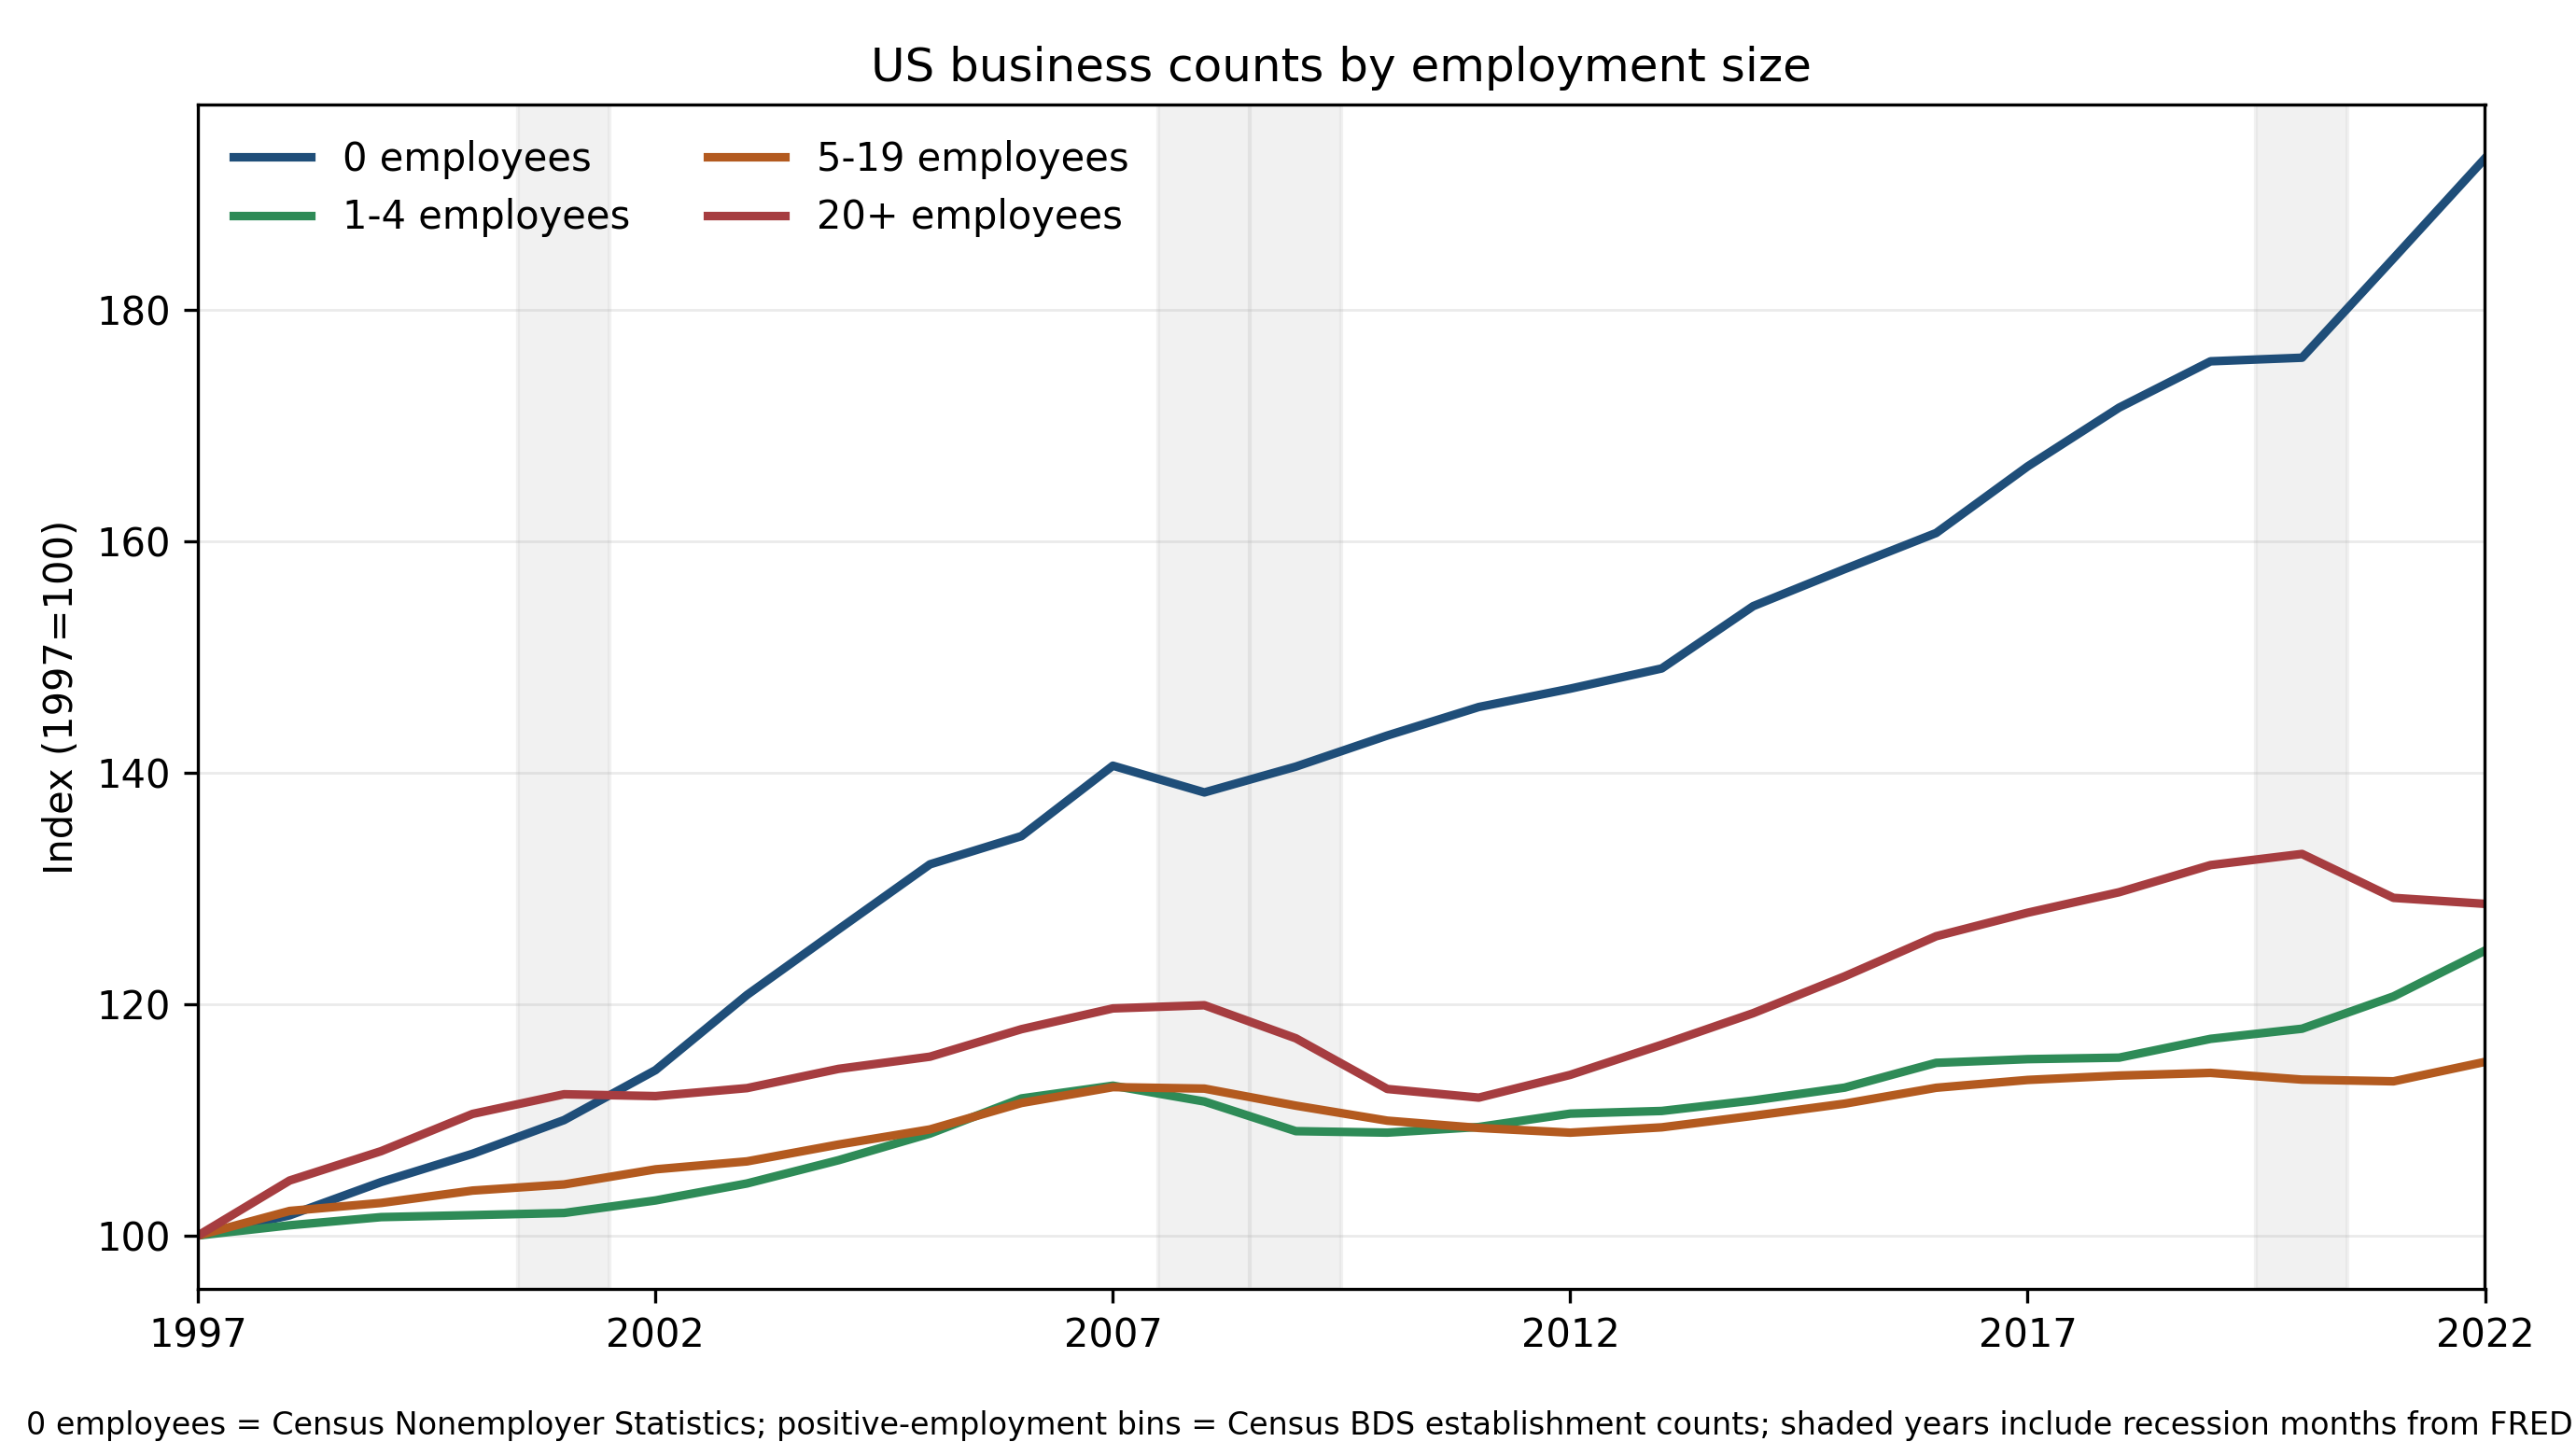
\includegraphics[width=0.92\textwidth]{us_business_counts_by_size_indexed.png}
\caption{U.S. business counts by employment size, indexed to 2007 = 100. The
zero-employee margin is comparatively resilient in the Great Recession, while
employer establishments contract.}
\label{fig:us_business_counts_by_size}
\end{figure}

The stock evidence is complemented by flow evidence. Using Census Business
Formation Statistics, total business applications decline over the 2007--2010
window, while high-propensity applications decline much more sharply. In our
side evidence, total applications fall by about 5.8 percent and
high-propensity applications fall by about 22.1 percent, producing a sizable
decline in the high-propensity share of all applications. This pattern aligns
with the broader startup-dynamics literature. \citet{sedlacek_sterk_2017} show
that startup cohorts born in weak aggregate conditions are persistently smaller
and have lower growth potential. \citet{haltiwanger_etal_2013} show that
startups and young firms are disproportionately important for job creation,
while \citet{fort_etal_2013} and \citet{zarutskie_yang_2017} document that
young firms were especially weak during the Great Recession. Recession
conditions may therefore preserve or increase low-scale entry while
simultaneously weakening the formation of employer firms with stronger growth
prospects. Figure~\ref{fig:us_business_applications} places this point on the
flow margin.

\begin{figure}[t]
\centering
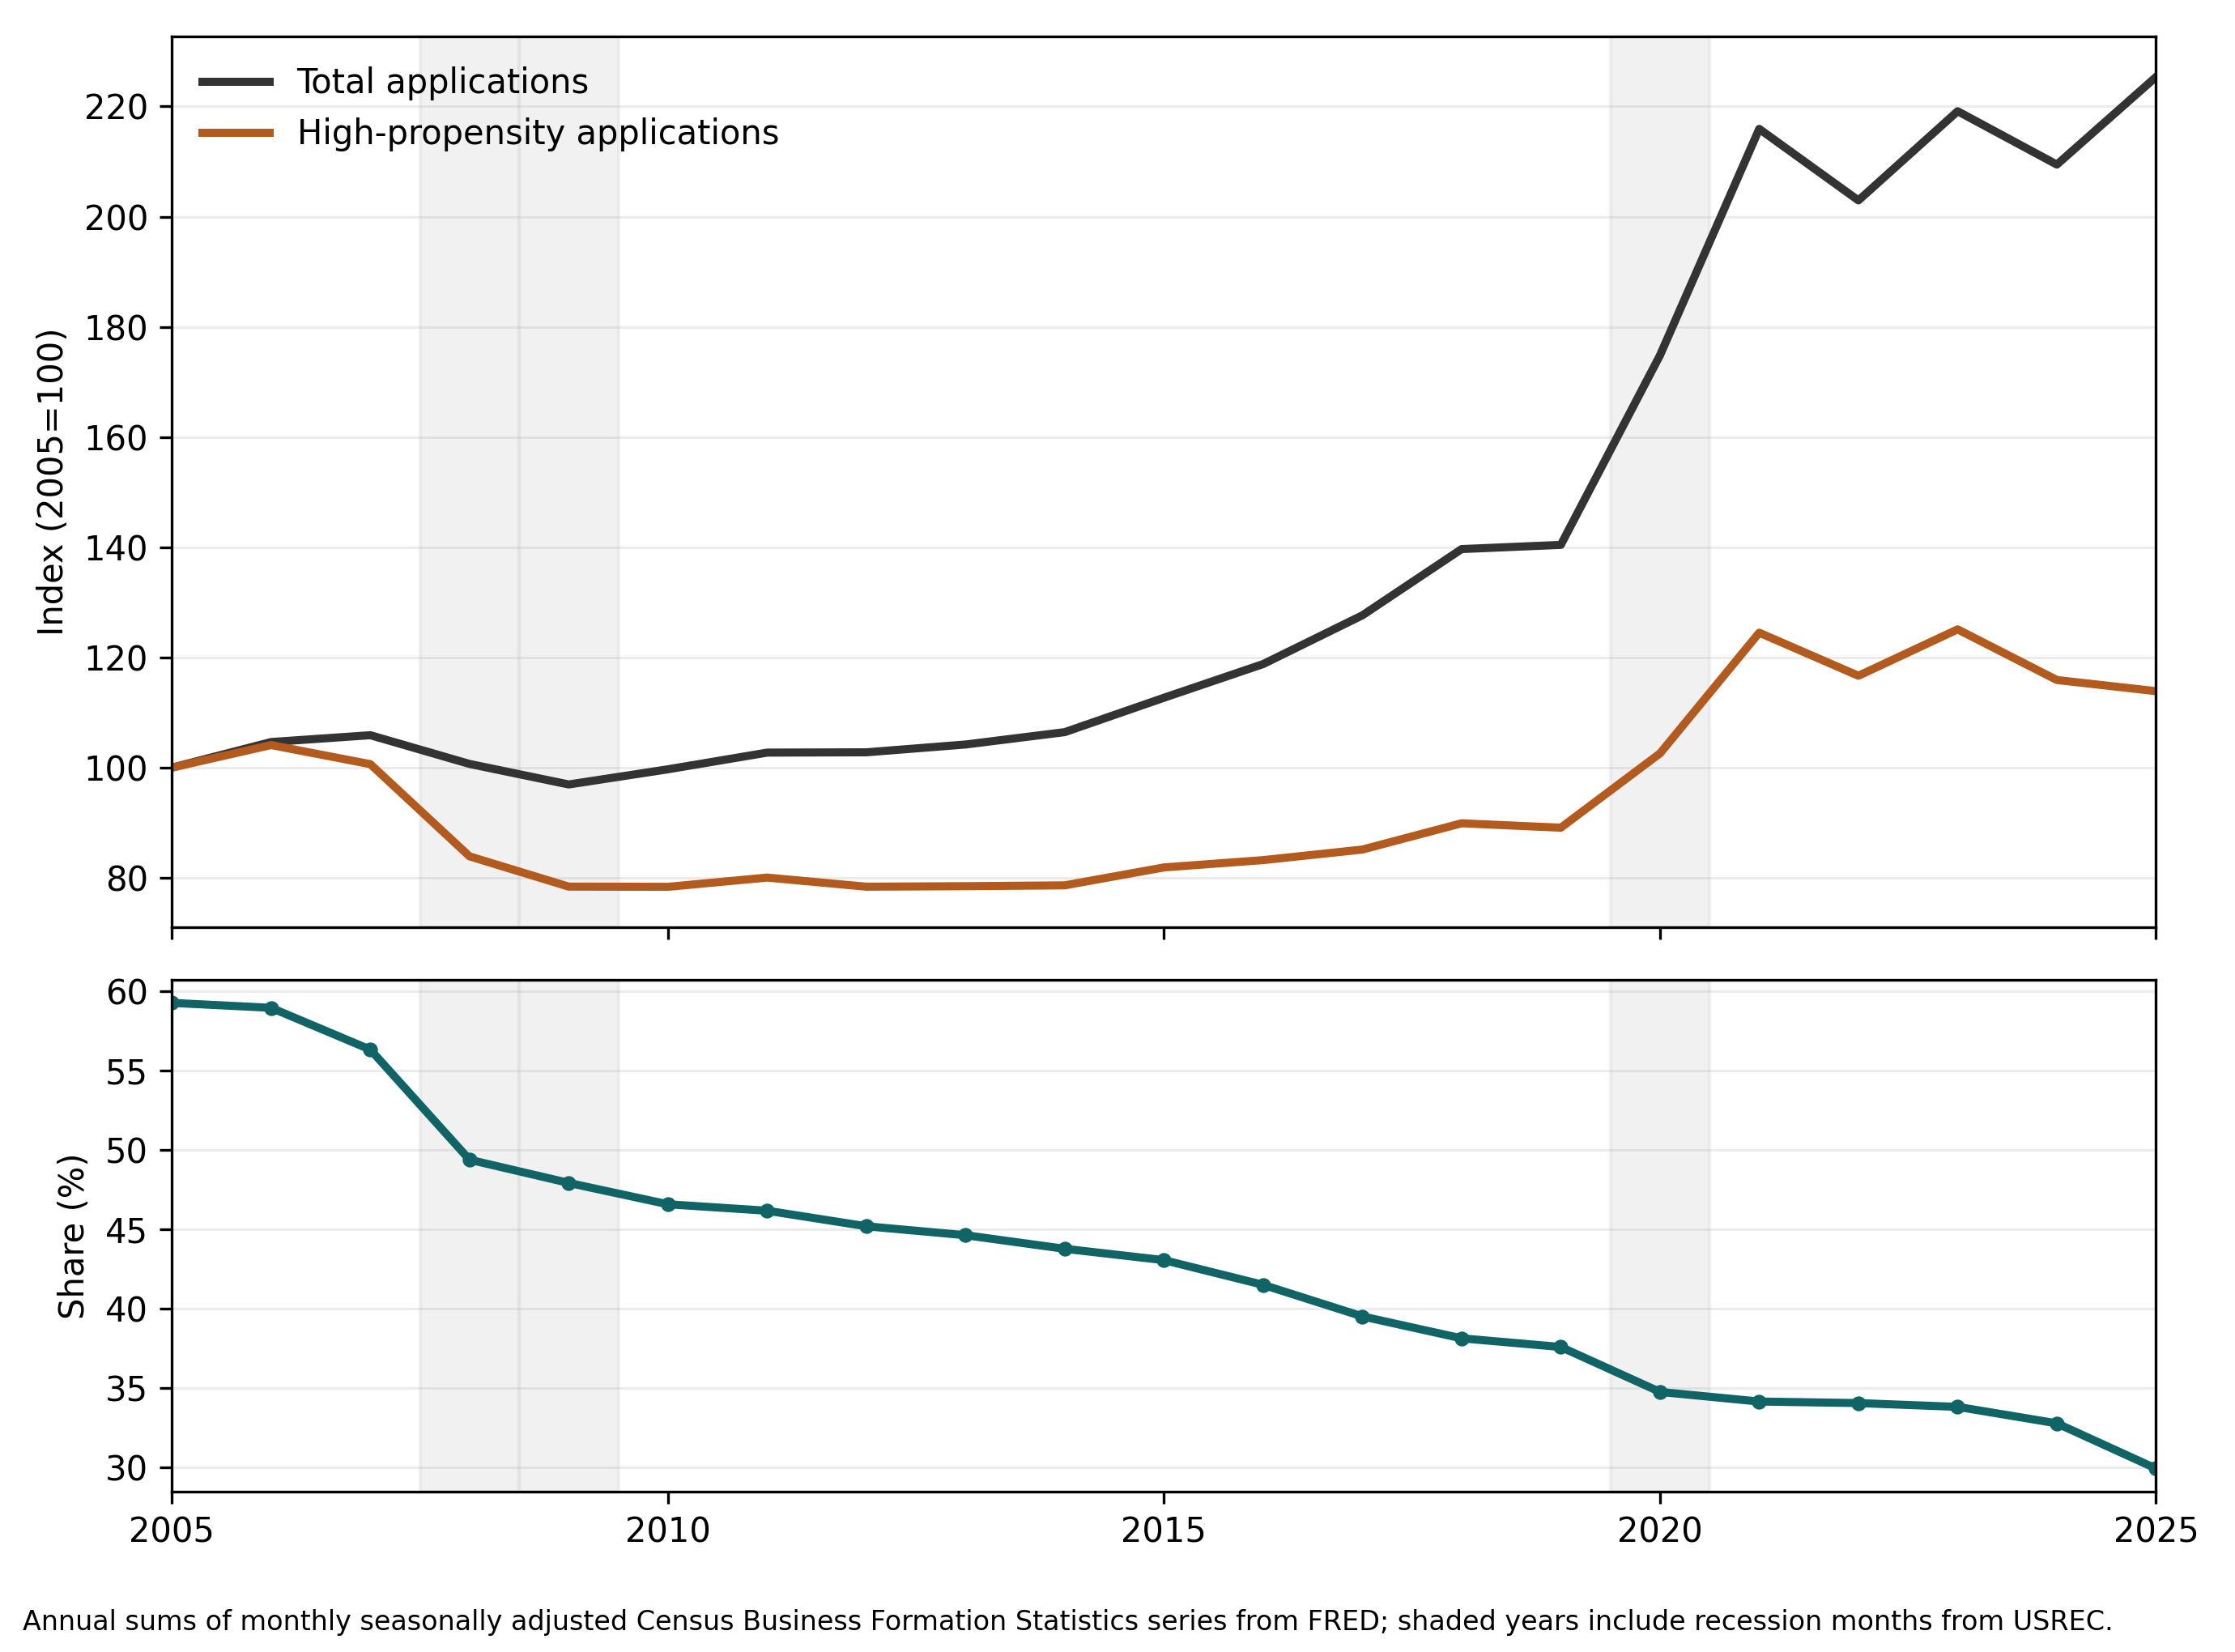
\includegraphics[width=0.92\textwidth]{us_business_applications_indexed.png}
\caption{U.S. business applications, indexed to 2007 = 100. Total applications
decline over the recession window, and high-propensity applications fall much
more sharply.}
\label{fig:us_business_applications}
\end{figure}

That distinction is important because low-scale business ownership is not the
same thing as employer-firm creation. \citet{fairlie_miranda_2016} show that
most nonemployer startups do not hire, and that transitions from nonemployer to
employer status are concentrated among more growth-oriented businesses.
\citet{hurst_pugsley_2011} likewise show that the typical small business is not
organized around innovation or expansion. A rise in zero-employee activity
should therefore not be read mechanically as evidence of greater productive
dynamism. More generally, the recession evidence suggests that the relevant
empirical comparison is across margins: own-account or zero-employee business
activity, employer-oriented startup formation, and entrant scale or growth
potential.

Against this background, we develop a heterogeneous-agent occupational-choice
model with entrepreneurial ability, human capital, search frictions,
separation risk, and unemployment insurance. Employment relationships are
valuable but risky. Unemployment insurance partly insures the downside of job
loss, but it also changes the return to waiting for wage work rather than
creating a business immediately. Entrepreneurship is therefore an endogenous
response to labor-market risk, incomplete insurance, and heterogeneity in
productive ability. This approach is closely related to the occupational-choice
and entrepreneurial heterogeneity literatures associated with
\citet{buera_2009}, \citet{cagetti_denardi_2006}, and \citet{poschke_2013},
but it adds an explicit distinction between entrepreneurship chosen with and
without a viable employment relationship. The model therefore allows downturns
and policy changes to affect not only the entrepreneurship rate, but also the
composition of entrepreneurs and the scale of the firms they operate.

The paper makes three contributions. First, it provides a structural definition
of necessity entrepreneurship that maps directly into state-contingent
occupational choice. Second, it embeds that definition in a quantitative
framework with heterogeneous education, entrepreneurial ability, search
frictions, and social insurance, allowing the model to speak jointly to entry,
firm scale, and labor-market conditions. Third, it interprets necessity
entrepreneurship as a margin of misallocation: weak outside options can push
some households into business ownership even when their productivity is better
deployed in paid employment. In that sense, the key issue is not only how much
entrepreneurship an economy generates, but what type of entrepreneurship it
generates.

This perspective matters for policy. Changes in unemployment insurance need not
move all entrepreneurship measures in the same direction. A more generous
safety net may reduce low-scale necessity entry without reducing productive
dynamism if it improves worker-firm matching and lowers business creation driven
by weak outside options rather than genuine entrepreneurial comparative
advantage. For the same reason, recession-style comparative statics should be
judged by whether they reproduce the observed compositional shift toward
zero-employee activity and away from employer-oriented formation, rather than
by whether they move a single aggregate entrepreneurship statistic in
isolation.

The remainder of the paper proceeds as follows. Section 2 discusses the related
literature. Section 3 presents the model environment. Section 4 characterizes
household behavior and equilibrium. Section 5 describes the calibration.
Section 6 presents the baseline results, Section 7 studies the policy
counterfactuals, and Section 8 concludes.
